\section{Sitio Oficial Nuevo Lourdes}

Esta es una guia basica para la edición y publicación de contenido en este sitio web, los resultados seran visibles en el siguiente link \url{https://nuevolourdes.github.io/}.

Todos los archivos presentes en esta entrega deberán ser editados con un editor de texto convencional, algunos ejemplos de estos son:

\begin{itemize}
  \item notepad
  \item notepad++
  \item sublime text
  \item visual studio code
\end{itemize}

Todos estos editores se encuentran disponibles completamente gratis para todos los sistemas operativos, Windows, Mac OS y Linux.

\subsection{Obteniendo Archivos del Sitio}

Para obtener los archivos del sitio para modificarlo, es necesario tener la ultima versión de \texttt{git} instalada en su computadora, a continuación se presentan guías para hacerlo en distintos sistemas operativos, el sistema recomendado es Ubuntu.

\begin{itemize}
\item Windows: \href{https://git-scm.com/download/win}{Descargar aquí}
\item Ubuntu: \href{https://git-scm.com/book/es/v1/Empezando-Instalando-Git\#Instalando-en-Linux}{Seguir guia}
\end{itemize}

Luego de instalar \texttt{git} deberíamos de tener una consola especial llamada \texttt{git Bash} en el caso de Windows, en Linux se puede utilizar la consola usual para los siguientes pasos, deberá ejecutar los siguientes comandos (cada \$ es un comando distinto, no incluirlo al digitar los comandos):

\begin{codeblock}{bash}
$ git clone https://github.com/nuevolourdes/sitio
$ cd sitio
$ git submodule add -b master \
https://github.com/nuevolourdes/nuevolourdes.github.io.git public
\end{codeblock}

Luego de ejecutar estos comandos se deberá tener un folder cuyos contenidos serán parecidos a lo siguiente bloque, (se han dejado de fuera los folders que no editaremos o no importan para los propositos de esta guía), dentro de estos se definen todo el contenido del sitio en texto plano en archivos ya sea de formato \texttt{.md} o formato \texttt{.yaml}:

\begin{codeblock}{bash}
.
./auto
./config.toml
./content
./data
./deploy.sh
./public
./static
./themes
\end{codeblock}

\subsection{Añadiendo Nuevo Contenido}

Para añadir nuevo contenido o remover contenido viejo, deberemos tener instalado un programa llamado \texttt{hugo}, descarga el archivo respectivo para poder correrlo en tu sistema operativo:

\begin{itemize}
\item Windows: \href{https://github.com/gohugoio/hugo/releases/download/v0.52/hugo_0.52_Windows-64bit.zip}{Hugo para Windows}
\item Ubuntu: \href{https://github.com/gohugoio/hugo/releases/download/v0.52/hugo_0.52_Linux-64bit.deb}{Hugo para Linux}
\end{itemize}

\subsubsection{Cambiando Contenido de Página
frontal}

\begin{codeblock}{bash}

data/
  carousel/
    confiable.yaml
    valores.yaml
  features/
    ambiente.yaml
    educacion.yaml
    valores.yaml
\end{codeblock}

Podemos cambiar el contenido de la pagina frontal en varios aspectos, dentro del folder \texttt{carousel} se cambian los contenidos ilustrados por la figura~\ref{fig:carousel}:

\begin{figure}[htbp]
\centering

\includegraphics[width=12cm]{../static/img/carousel.png}
\caption{carousel}
\label{fig:carousel}
\end{figure}

Dentro el folder \texttt{features} se cambian los aspectos de la página ilustrados por la figura~\ref{fig:features}, dentro de estos archivos se encontraran las definiciones de visión, misión y valores, los cuales podrán ser editados y guardados para actualizar el sitio:

\begin{figure}[htbp]
\centering
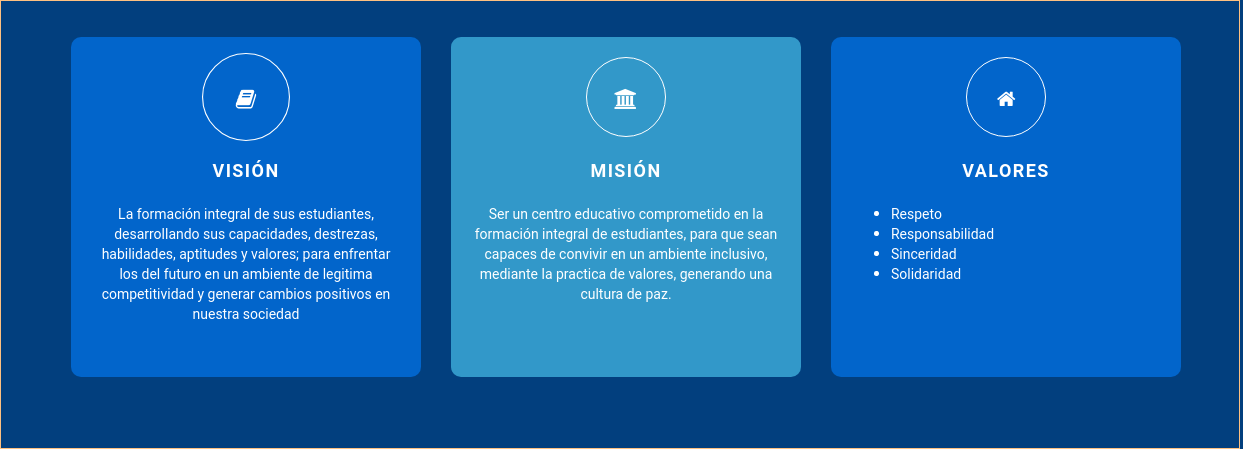
\includegraphics[width=12cm]{../static/img/features.png}
\caption{features}
\label{fig:features}
\end{figure}

\subsubsection{Añadiendo Noticias}

\begin{figure}[htbp]
\centering
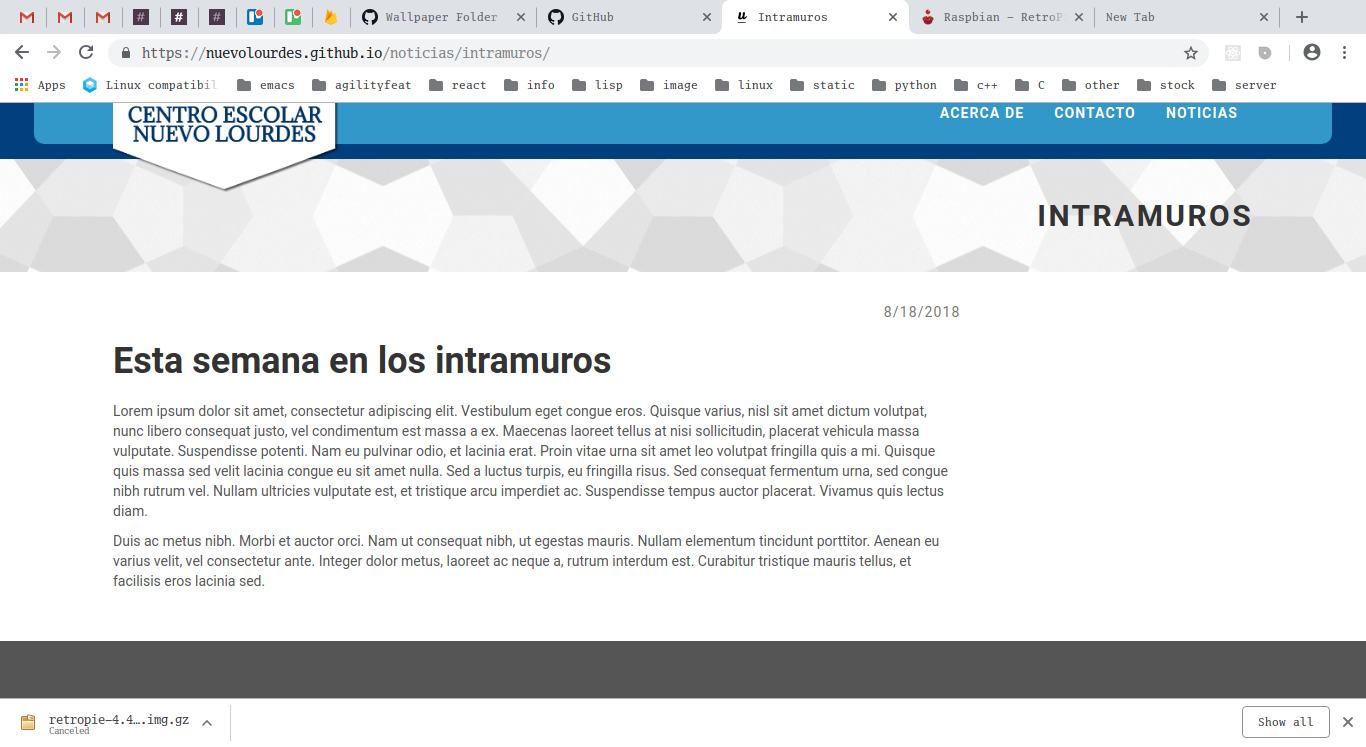
\includegraphics[width=12cm]{../static/img/noticia.png}
\caption{Ejemplo de una Noticia}
\label{fig:noticia}
\end{figure}

Podemos hallar el contenido actual bajo esta estructura, en el folder
\texttt{contents}:

\begin{codeblock}{bash}

content/
  acercade.md
  noticias/
    entreganotas.md
    intramuros.md
    nuevopost.md
\end{codeblock}

Podemos crear un nuevo archivo con extension \texttt{.md} para crear una
nueva página con el contenido de noticias, podemos simplemente copiar
uno existente, renombrar y editar los contenidos del nuevo archivo, los
contenidos se verán a continuación.

\begin{codeblock}{bash}
---
title: "Vacaciones"
date: 2018-08-19T17:53:29-06:00
draft: false
type: "blog"
---

# Vacaciones semana santa

Sed dolor sapien, rhoncus nec urna vitae, rhoncus congue urna. 
Duis quis vehicula massa. Ut scelerisque consectetur justo. 
Nam in libero at dui lacinia scelerisque molestie id eros. 
Curabitur est felis, viverra in mauris eu, tristique efficitur 
neque. Vestibulum lorem ex, consectetur consequat justo ac, scelerisque 
dignissim sapien. In eu lobortis tellus. 

![texto](./img/unaimagen.jpg)
\end{codeblock}

El texto bajo \texttt{title}, sera el titulo de nuestra noticia, \texttt{date} la fecha, \texttt{draft} indica si este es un borrador, siempre deberá ser \texttt{false} para asegurarnos de que nuestras noticias se publiquen siempre, finalmente en la configuración tenemos \texttt{type}, el cual en el caso de las noticias deberá estar siempre en \texttt{blog}.

Podemos añadir imágenes a la carpeta \texttt{static/img/} dentro de la carpeta principal, luego podemos incluir las imágenes en las noticias de la forma que se utiliza arriba.

\subsubsection{Markdown}

este es el formato en la que la mayoria de contenido estara escrito, se
explicara brevemente que significa cada elemento en este formato, a
continuación un ejemplo:

\begin{codeblock}{C}

# Este es un titulo
## Esto es un subtitulo
### Esto es un subsubtitulo

===

El bloque de arriba "===" indica una linea separadora en nuestro 
contenido, también podemos crear listas:

* este es un elemento
* este es otro elemento
* este es un tercer elemento

===

Para insertar imágenes podemos hacerlo fácilmente
usando el siguiente formato:

![texto auxiliar](/url/o/ruta/al/archivo)

Si hacemos esto sin el signo de exclamación,
el resultado final será un link a la imagen,
es decir, esta no se mostrara.

===

esto es texto en **negrita** y esto es texto en *cursivo*

<p>
  como una función avanzada también podemos utilizar 
  HTML dentro de esta versión de markdown.
</p>
\end{codeblock}

Para una lista más comprensiva de las funcionalidades del formato \texttt{markdown} se recomienda revisar este sitio: \url{https://markdown.es/sintaxis-markdown/}

\subsection{Probando cambios antes de subirlos}

Para probar los cambios, se puede utilizar \texttt{hugo}, de la siguiente forma:

\begin{codeblock}{bash}

$ hugo serve
\end{codeblock}

Este comando ocasionara que los archivos sean interpretados y que el resultado final sea colocado en la carpeta \texttt{public}, también actuara como un servidor local, el cual podremos ver funcionando en la consola desde la cual ejecutamos el comando, a continuación, se puede dirigir a la dirección \url{http://localhost:1313} para ver el resultado, cualquier cambio que se haga mientras corre el servidor será automaticamente actualizado en la versión local, cuando se este satisfecho, es hora de subir cambios.

\subsection{Subiendo cambios}


Subir los cambios es muy sencillo, solo se requiere ejecutar el siguiente comando, luego de eso los cambios estarán arriba en cuestión de minutos:

\begin{codeblock}{bash}
$ bash ./deploy.sh
\end{codeblock}

Luego se puede navegar a \url{https://nuevolourdes.github.io/}, para observar el sitio actualizado.


%%% Local Variables:
%%% mode: latex
%%% TeX-master: "reporte"
%%% End:
